% Software Development for Mobile Devices
\documentclass[11pt,english,numbers=endperiod,parskip=half]{scrartcl}

\usepackage{color}
\usepackage{graphicx}
\usepackage{minted}
\usepackage{fancyhdr}

\pagestyle{fancy}

\rhead{Daniel Parker - 971328X}
\lhead{COS30017 - Software Development for Mobile Devices}

\title{Assignment 02}
\subtitle{COS30017 - Software Development for Mobile Devices}
\author{Daniel Parker 971328X}

\date{\today}

\begin{document}
\maketitle
\thispagestyle{empty}

\section{Task 1}
\subsection{Three activities}
\raggedright
Activities are connected using intents. Intents allow new activities to be launched on events that occur in the main activity. Furthermore, data can be passed between the activities if necessary to give the activity context. The main activity in this app, \textit{MainActivity.java} uses intents to launch the other two activites, \textit{HeightActivity.java} and \textit{TempActivity.java}. If the user presses the back button in one of the second two activities they will return to the \textit{MainActivity.java}

\inputminted[firstline=40,lastline=50]{java}{../../Apps/Converters/app/src/main/java/au/net/danielparker/converters/MainActivity.java}

When one of the form-based activity's orientation changes, the \textit{onSaveInstanceState} event is called. By overriding that method, the form data can be saved and then retrieved after the activity is recreated by overriding \textit{onRestoreInstanceState} and restoring that data to the correct views in the activity.

\inputminted[firstline=37,lastline=58]{java}{../../Apps/Converters/app/src/main/java/au/net/danielparker/converters/HeightActivity.java}

\subsection{Layouts}
\subsubsection{activity\_main.xml}
\inputminted{xml}{../../Apps/Converters/app/src/main/res/layout/activity_main.xml}
\subsubsection{activity\_height.xml}
\inputminted{xml}{../../Apps/Converters/app/src/main/res/layout/activity_height.xml}
\subsubsection{activity\_temp.xml}
\inputminted{xml}{../../Apps/Converters/app/src/main/res/layout/activity_temp.xml}

\subsection{Screenshots}
The following two screenshots show how the orientation change doesn't cause the data in the activity to disappear, due to it being passed in the state change bundle and then restored to the activity when it is recreated.

\setlength\fboxsep{0pt}
\setlength\fboxrule{0.5pt}
\centering{
	\fbox{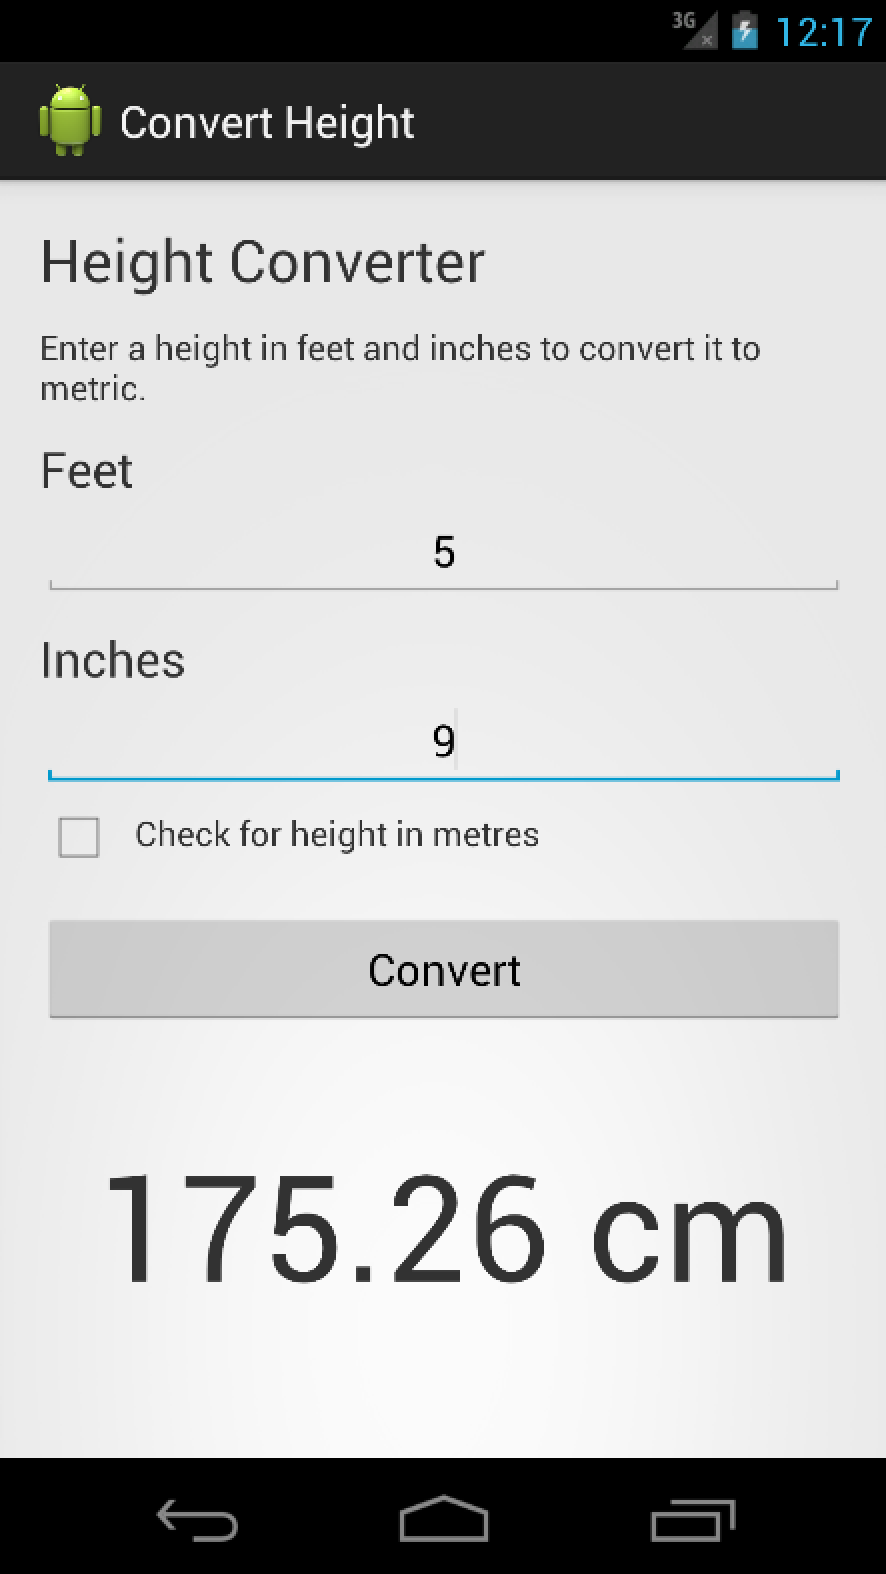
\includegraphics[width=5cm]{images/height-p.png}}
}\\
\bigskip
\centering{
	\fbox{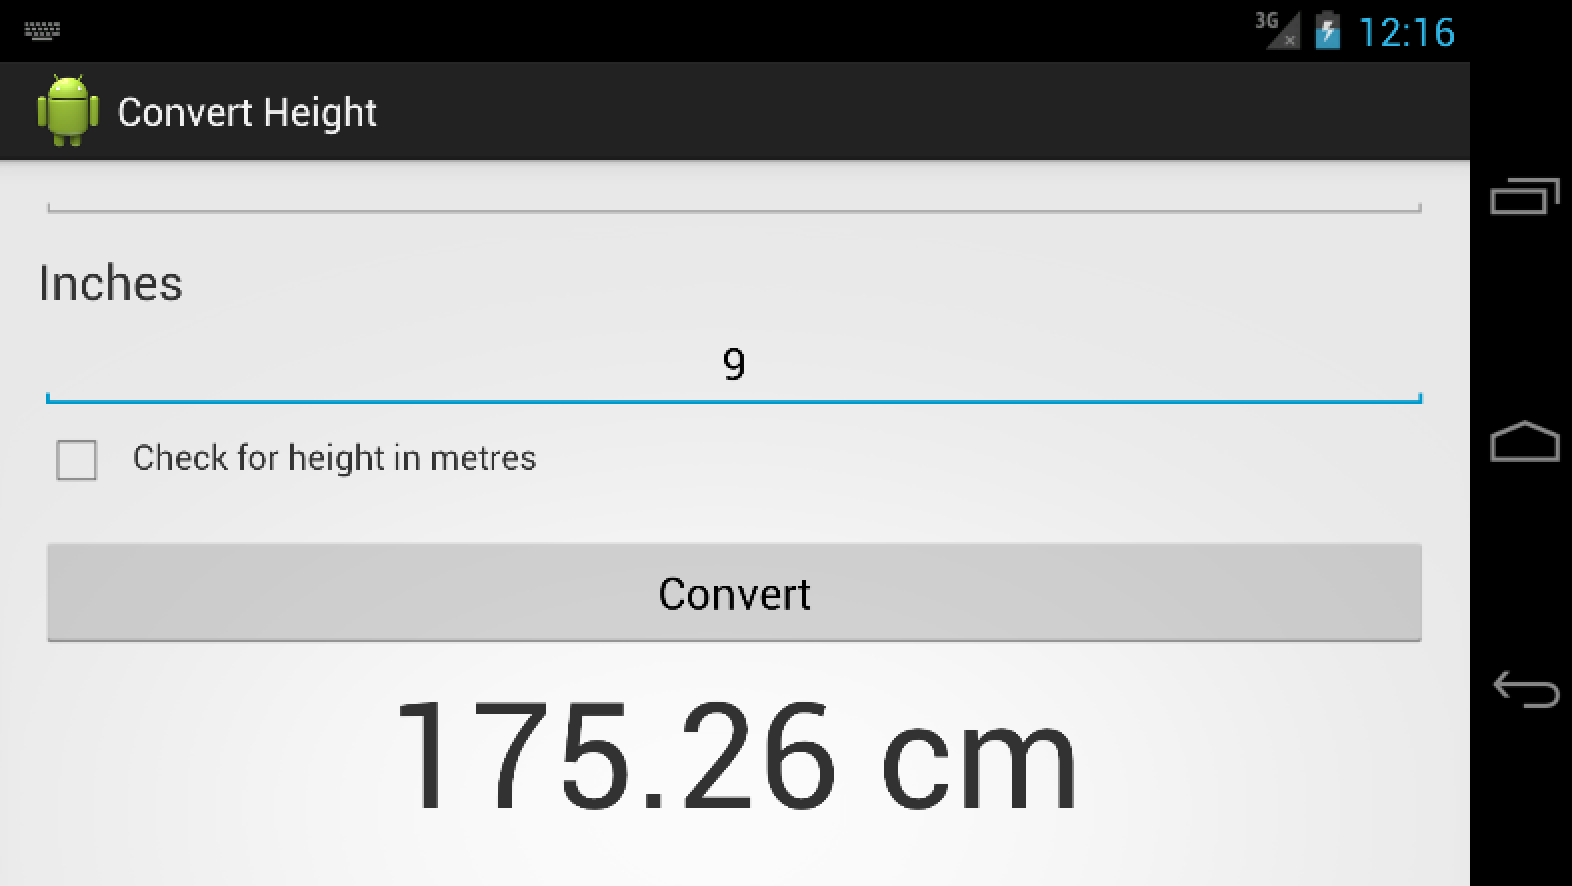
\includegraphics[width=8cm]{images/height-l.png}}
}\\

\subsection{Task 2}
In this app, the image and description resource IDs are passed through the intent to the recieving Activity which then sets the resource using those IDs.
\subsection{ImageGallery.java}
\inputminted[firstline=41,lastline=83]{java}{../../Apps/ImageIntent/app/src/main/java/au/net/danielparker/imageintent/ImageGallery.java}
\subsection{ImageActivity.java}
\inputminted[firstline=51,lastline=59]{java}{../../Apps/ImageIntent/app/src/main/java/au/net/danielparker/imageintent/ImageActivity.java}

\subsection{Layouts}
\subsubsection{activity\_image\_gallery.xml}
\inputminted{xml}{../../Apps/ImageIntent/app/src/main/res/layout/activity_image_gallery.xml}

\subsubsection{activity\_image.xml}
\inputminted{xml}{../../Apps/ImageIntent/app/src/main/res/layout/activity_image.xml}

\subsection{Screenshots}
\centering{
	\fbox{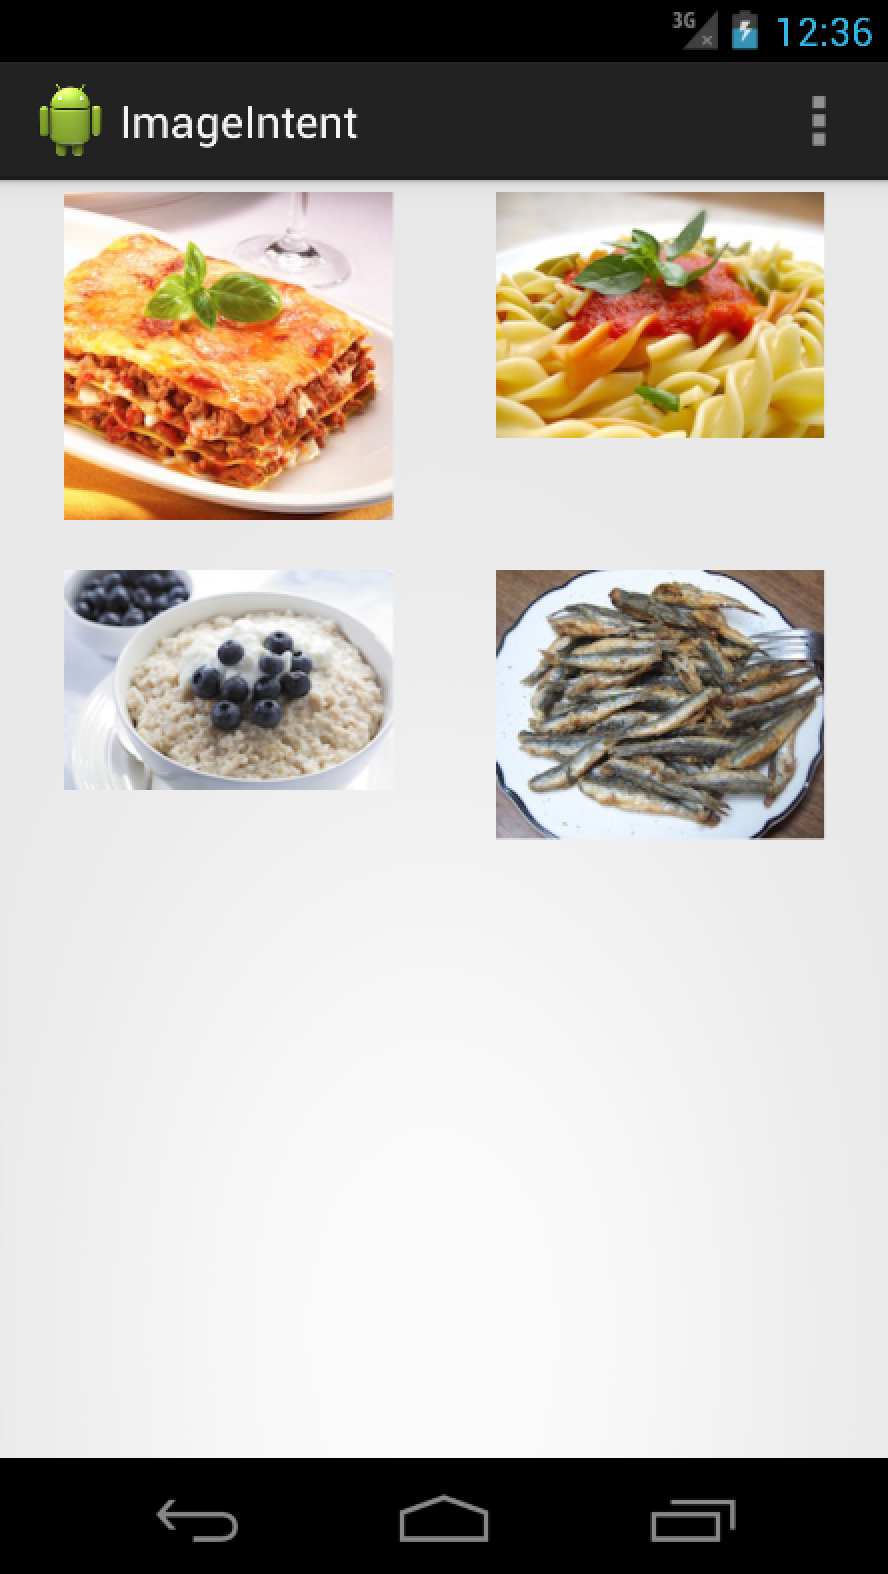
\includegraphics[width=5cm]{images/gallery.png}}
}\\
\bigskip
\centering{
	\fbox{
\includegraphics[width=5cm]{images/lasagna.png}}
}\\
\bigskip
\centering{
	\fbox{
\includegraphics[width=5cm]{images/pasta.png}}
}\\

\section{Task 3}


\end{document}
